% \documentclass[oneside]{report}
\documentclass[oneside,final,14pt,a4paper]{extreport}
% \documentclass[journal,onecolumn,a4paper,12pt]{IEEEtran}
\usepackage[T2A]{fontenc}


\usepackage{vmargin}
\setpapersize{A4}
\setmarginsrb{2.5cm}{2cm}{2cm}{2cm}{0pt}{10mm}{0pt}{13mm}
\usepackage{setspace}
\sloppy
\setstretch{1.5}
\usepackage{indentfirst}
\parindent=1.25cm

%%%%% ADDED TO SUPPORT TT BOLD FACES %%%%
\DeclareFontShape{OT1}{cmtt}{bx}{n}{<5><6><7><8><9><10><10.95><12><14.4><17.28><20.74><24.88>cmttb10}{}
\renewcommand{\ttdefault}{pcr}
%%%%% END %%%%%%%%%%%%%%%%%%%%%%%%%%%%%%% 
\usepackage{atbegshi,picture}
\AtBeginShipout{\AtBeginShipoutUpperLeft{%
  \put(\dimexpr\paperwidth-1cm\relax,-1.5cm){\makebox[0pt][r]{
\includegraphics[width=3cm]{figs/inno}}}%
}}


\usepackage[english]{babel}
\usepackage[backend=biber,style=ieee,autocite=inline]{biblatex}
\bibliography{ref.bib}
\DefineBibliographyStrings{english}{%
  bibliography = {References},}
\usepackage{blindtext}
\usepackage{pdfpages}
\newenvironment{bottompar}{\par\vspace*{\fill}}{\clearpage}
\usepackage{amsmath,amsfonts}
\usepackage{url}

\usepackage{amsthm}
\newtheorem{theorem}{Theorem}
\newtheorem{corollary}{Corollary}
\newtheorem{lemma}{Lemma}
\newtheorem{proposition}{Proposition}
\theoremstyle{definition}
\newtheorem{definition}{Definition}
\theoremstyle{remark}
\newtheorem*{remark}{Remark}
\theoremstyle{remark}
\newtheorem*{example}{Example}


\usepackage{titlesec}
\usepackage{float}
\usepackage{graphicx}
\graphicspath{{figs/}} %path to images
\usepackage{array}
\usepackage{multirow,array}
\usepackage{caption}
\usepackage{subcaption}
\usepackage{hyperref}
\usepackage{paralist}
\usepackage{listings}
\usepackage{zed-csp}
\usepackage{fancyhdr}
\usepackage{csquotes}
\usepackage{color}
\usepackage{anyfontsize}
\usepackage{mathptmx}
\usepackage{t1enc}

\usepackage{chngcntr}
\usepackage{upgreek} 
\usepackage{bm}
\usepackage{hyperref}
\usepackage{setspace}
\usepackage{booktabs}
\usepackage{multirow}
\usepackage{longtable}
\usepackage[font=singlespacing, labelfont=bf]{caption}
\counterwithout{table}{chapter}
\renewcommand{\thetable}{\Roman{table}}
%Hints
\newcommand\pic[1]{(Fig. \ref{#1})} %Ref on figure
\newcommand\tab[1]{(Tab. \ref{#1})} %Ref on table

\setlength{\headheight}{32.0976pt}
\usepackage{enumitem}
\newlist{inlinelist}{enumerate*}{1}
\setlist*[inlinelist,1]{%
  label=(\arabic*),
}

\setcounter{secnumdepth}{4}
% ->
% \captionsetup[table]{labelfont={normalfont}, name={TABLE}, labelsep={newline}}
\counterwithout{table}{chapter}
\renewcommand{\thetable}{\Roman{table}}
\setlength{\parindent}{2em} 
\DeclareCaptionLabelSeparator{figSep}{.\quad}
% ->
% \captionsetup[figure]{labelfont={normalfont}, name={Fig.}, labelsep=period}
\counterwithout{figure}{chapter}

\titleformat{\section}[hang]{\fontsize{20}{24}\selectfont\filcenter}{\Roman{section}}{1em}{}
\titleformat{\subsection}[hang]{\itshape}{\Alph{subsection}.}{1em}{}[]
\titleformat{\subsubsection}[runin]{\itshape}{\arabic{subsubsection})}{1em}{}[$:$]
\titlespacing{\subsubsection}{1em}{1em}{1em}
\titleformat{\paragraph}[runin]{\itshape}{\alph{paragraph})}{1em}{}[$:$\quad]
\titlespacing{\paragraph}{2em}{1em}{1em}

\pagestyle{fancyplain}

% remember section title
\renewcommand{\chaptermark}[1]%
	{\markboth{\chaptername~\thechapter~--~#1}{}}

% subsection number and title
\renewcommand{\sectionmark}[1]%
	{\markright{\thesection\ #1}}

\rhead[\fancyplain{}{\bf\leftmark}]%
      {\fancyplain{}{\bf\thepage}}
\lhead[\fancyplain{}{\bf\thepage}]%
      {\fancyplain{}{\bf\rightmark}}
\cfoot{} %bfseries


\newcommand{\dedication}[1]
   {\thispagestyle{empty}
     
   \begin{flushleft}\raggedleft #1\end{flushleft}
}

\begin{document}
\setboolean{@twoside}{false}
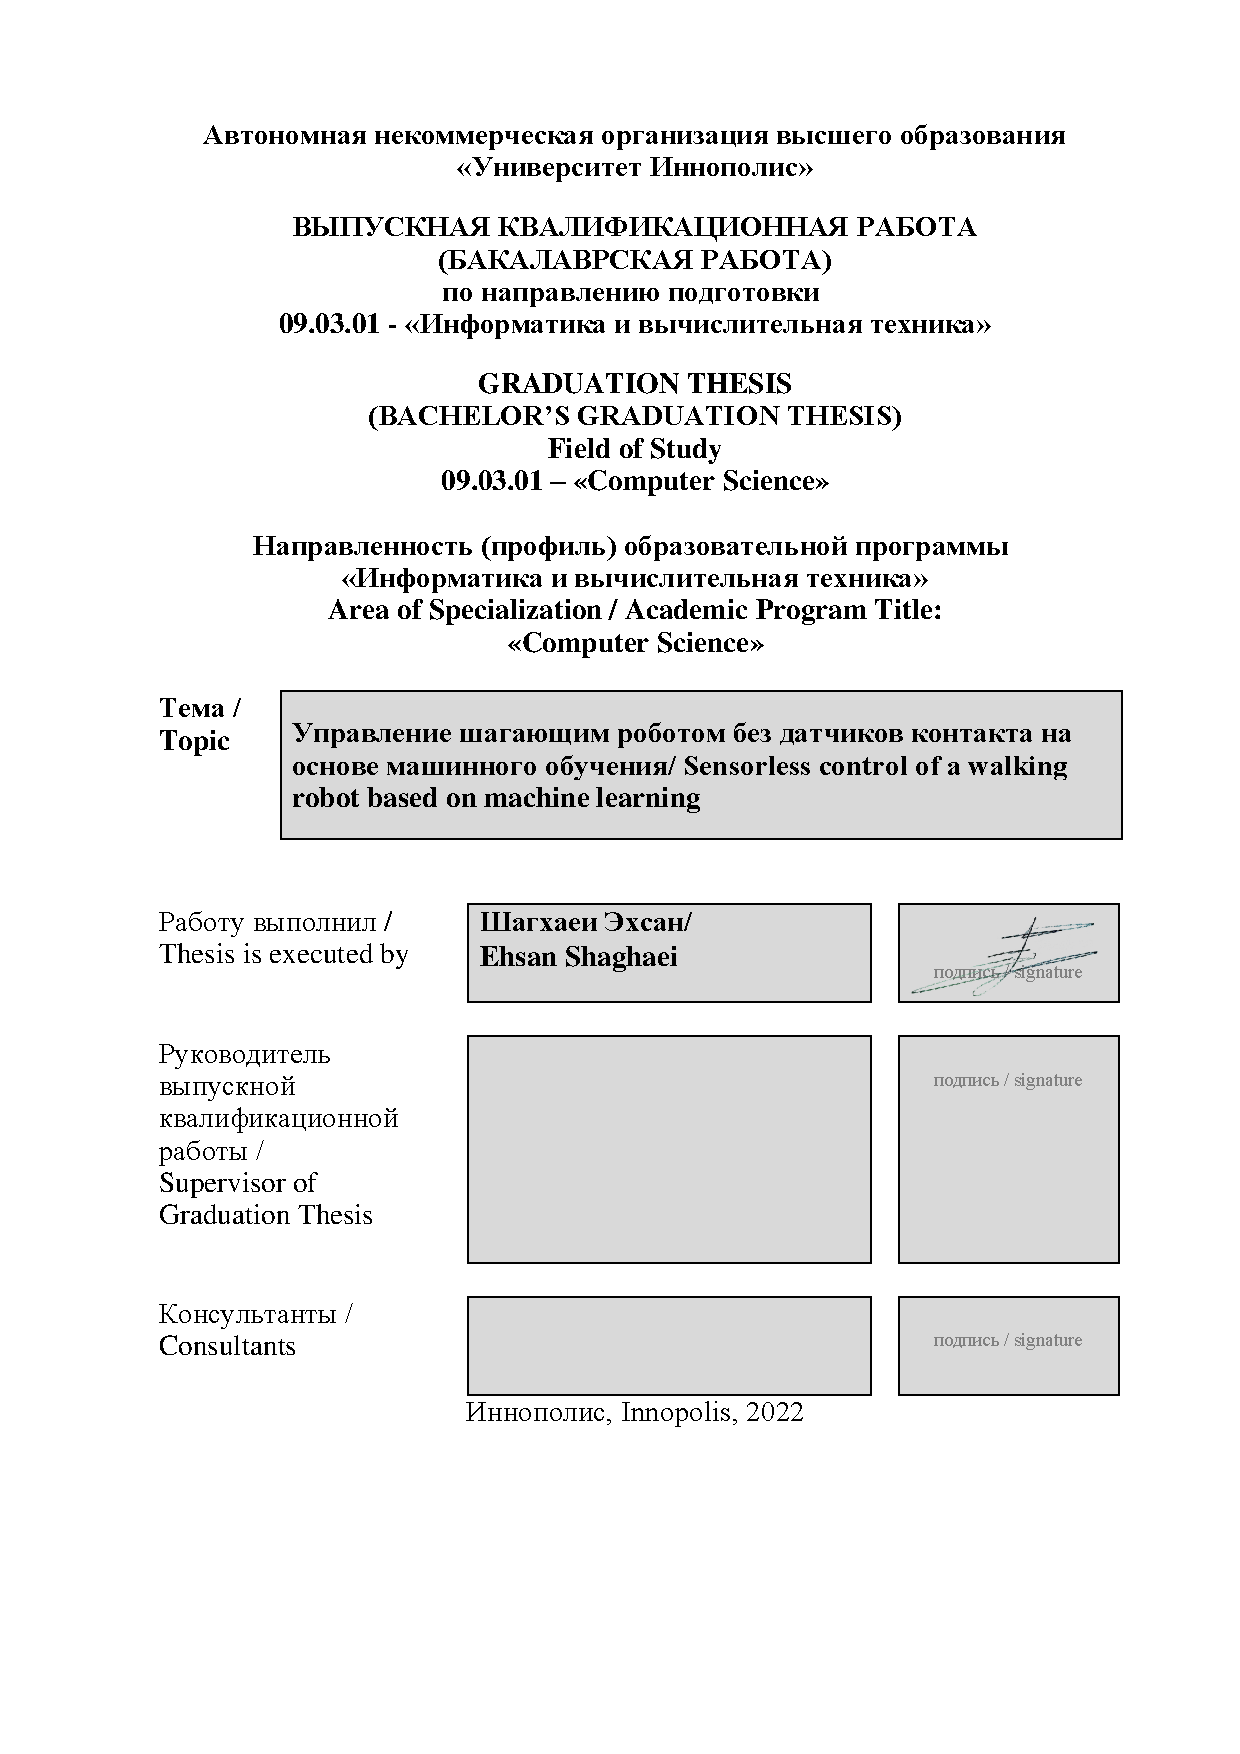
\includepdf[pages=-, offset=75 -75]{title.pdf}
\tableofcontents
\listoftables
\listoffigures


\newpage
\begin{abstract}

% Background: Describe the problem space you are working on, why it is important for the community, and why there is a need for this research.  
Bipedal robots collect data by internal sensors, and it is common to get basic data about the surroundings of the robot environment.
% Objective: State your research project objective, research questions, or hypotheses.
This paper is focused on problem of using the environmental sensor data in order to predict contact interaction scenario of a bipedal robot.
% Methods: Introduce the study design and methods you used for this work. 
Prediction of contact interaction scenario has been proposed. Our methodology utilizes a architecture of fully connected neural networks to utilize environmental data for predicting contact interaction scenario.
% Results: Briefly state what you accomplished or found, especially as it pertains to the objective stated earlier. 
As result, Our model can predict predicting contact interaction scenario with
 {\color{red}XX
 \footnote{Draft note: \color{red}the red marked texts will be finalized after actual results}
% Implications: Identify 1–2 implications or contributions of this work.
 }. The utilization of this method can enhance the performance of contact interaction scenario improvisation, such as slipping or take off from the supporting surface for bipedal robots.




\end{abstract}
% Depend on above part
% \setcounter{page}{6}
% \chapter{Introduction}
\label{chap:intro}
\chaptermark{Optional running chapter heading}
\section{Spacing \& Type}
\label{sec:section}

This is a section. This is a citation without brackets. and this is one with brackets \cite{A}. Multiple \cite{A,B,C} Here's a reference to a subsection: \ref{sec:subsection}. Citation of an online article \cite{D}. Citation of an online proceeding \cite{F}. The body of the text and abstract must be double-spaced except for footnotes or long quotations. Fonts such as Times Roman, Bookman, New Century Schoolbook, Garamond, Palatine, and Courier are acceptable and commonly found on most computers. The same type must be used throughout the body of the text. The font size must be 10 point or larger and footnotes\footnote{This is a footnote.} must be two sizes smaller than the text\footnote{This is another footnote.} but no smaller than eight points. Chapter, section, or other headings should be of a consistent font and size throughout the ETD, as should labels for illustrations, charts, and figures.

\subsection{Creating a Subsection}
\label{sec:subsection}

\subsubsection{Creating a Subsubsection}
\subsubsection{Creating a Subsubsection}
\subsubsection{Creating a Subsubsection}

\paragraph{This is a heading level below subsubsection}

And this is a quote: 
%
\begin{quote}
\blindtext
\end{quote}

\begin{figure}[hbt]
\centering

\includegraphics[]{figs/inno.png}
\caption{One kernel at $x_s$ (\emph{dotted kernel}) or two kernels at
$x_i$ and $x_j$ (\textit{left and right}) lead to the same summed estimate
at $x_s$. This shows a figure consisting of different types of
lines. Elements of the figure described in the caption should be set in
italics, in parentheses, as shown in this sample caption.}
\label{fig:example}
\end{figure}

This is a table:
% currsize is not set in the long table environment, so we need to set it before we set it up.
\makeatletter
\let\@currsize\normalsize
\makeatother

% tabular environments are set to be single-spaced in the  thesis class,  but long tables do not use tabular
% to get around this, set the spacing to single spacing at the start of the long table environment, and set it back to double-spacing at the end of it

\begin{longtable}{c|c|c}
\caption[This is the title I want to appear in the List of Tables]{This Is a Table Example} \label{tab:pfams} \\
\hline
A & B & C \\
\hline
\endfirsthead
\multicolumn{3}{@{}l}{} \\
\hline
A & B & C\\
\hline
\endhead
a1 & b1 & c1 \\
a2 & b2 & c2\\
a3 & b3 & c3\\
a4 & b4 & c4\\
\hline
\end{longtable}

The package ``upgreek'' allows us to use non-italicized lower-case greek letters. See for yourself: $\upbeta$, $\bm\upbeta$, $\beta$, $\bm\beta$. Next is a numbered equation:
\begin{align}
\label{eq:name}
\|\bm{X}\|_{2,1}={\underbrace{\sum_{j=1}^nf_j(\bm{X})}_{\text{convex}}}=\sum_{j=1}^n\|\bm{X}_{.,j}\|_2
\end{align}
The reference to equation (\ref{eq:name}) is clickable. 
\section[Theorems, Corollaries, Lemmas, Proofs, Remarks, Definitions and Examples]{Theorems, Corollaries, Lemmas, Proofs, Remarks, Definitions,and Examples}

\begin{theorem}
\label{thm:onlytheorem}
\blindtext
\end{theorem}

\begin{proof}
I'm a (very short) proof.
\end{proof}

\begin{lemma}
I'm a lemma.
\end{lemma}

\begin{corollary}
I include a reference to Thm. \ref{thm:onlytheorem}.
\end{corollary}

\begin{proposition}
I'm a proposition.
\end{proposition}

\begin{remark}
I'm a remark. 
\end{remark}

\begin{definition}
I'm a definition. I'm a definition. I'm a definition. I'm a definition. I'm a definition. I'm a definition. I'm a definition. I'm a definition. I'm a definition. I'm a definition. I'm a definition. 
\end{definition}

\begin{example}
I'm an example.
\end{example}


\section[Optional table of contents heading]{Section with\\ linebreaks in\\the
name}


\Blindtext[2]





% \chapter{Literature Review}
\label{chap:lr}

\vspace{4mm}
% Background: Describe the problem space you are working on, why it is important for the community, and why there is a need for this research.  
Humanoid bipedal robots are a rapidly growing area of research in the field of robotics. One of the primary challenges in developing these robots is achieving vertical balance, which has been identified as a key challenge in the literature \cite{Savin2017,cwc7139910}. To address this challenge, various approaches have been proposed, including the use of the contact-wrench cone \cite{cwc7139910} and the zero-moment point \cite{zmp1241826}. These approaches are based on the assumption that the contact interaction between the bipedal robot and the supporting surface can be accurately captured \cite{Savin8875522}.

\vspace{4mm}
% Objective: State your research project objective, research questions, or hypotheses.

Contact interaction with supporting surface can be captured by utilizing various learning methods such as reinforcement learning\cite{rl48550} and dense neural networks\cite{dnn8501736}. Aforementioned models needs data to train. This data can be obtained either through experiments or producing simulation-based data. 

\vspace{4mm}

The advantage to use machine learning for contact interaction with supporting surface capture with supporting surface is exclusion of unknown reaction forces from the dynamics equation of humanoid bipedal robots control system\cite{Savin8875522}. Formally, given the parameters $P$ I should introduce a projector matrix $\mathcal{P}$ into orthonormal basis $\mathcal{T}$ to the bipedal robot control system such:
% Methods: Introduce the study design and methods you used for this work
\vspace{4mm}

\begin{equation}
\label{eq:def} 
P = \{p_1, p_2, p_3, ...\} ; \forall p_i \in P, p_i \in \mathbb{R}^n
\\
\exists \mathcal{T} = \{ \tau_1,\tau_2,\tau_3,...,\tau_m \};  \mathcal{T} \in \mathbb{R}^{n \times m}; n,m \in \mathbb{Z}^{\ge0};\\ \forall \tau_p \tau_q \in \mathcal{T} :
\\
\tau_p^T \tau_q = 0 , \hspace{2mm}
     \tau_p^T \tau_q = 0 , \hspace{2mm}
     \|\tau_p\|=0 , \hspace{2mm}
     \|\tau_q\|=0 
     \\ \mathcal{P} \in \mathbb{R}^{n^2}
\end{equation}

\vspace{4mm}

 
 Learning methods predict components of projector matrix $\mathcal{P}$ to the bipedal robot control system by training to maximize reward function$(\lambda=-1)$\ref{eq:F} for reinforcement learning methods and minimize the loss  function$(\lambda=1)$ \ref{eq:F} for dense neural network methods. The key term which is the gap in current learning methods is predicting the \textbf{components} of contact interaction with supporting surface capture with supporting surface. The components are obtained 
 by singular-value-decomposition of projector matrix $\mathcal{P}$. My goal is to investigate if the components of the projection matrix $\mathcal{P}$ is predictable using learning methods and compare the accuracy of the prediction comparing to existing learning methods.

\vspace{4mm}

\begin{equation}
    \label{eq:F}
    \Psi = \lambda \sum_{p \in P} \| p - \mathcal{P}^* p\| ;
    \lambda = \begin{cases}
        1 \text{ Reinforcement learning methods}\\
        -1 \text{ Dense neural networks}
    \end{cases}
    % \caption{\mathcal{\mu}  defining reward/loss function}
\end{equation}

\vspace{4mm}

% Results: Briefly state what you accomplished or found, especially as it pertains to the objective stated earlier.
The optimization problem of maximizing the reward function in gradient ascent \cite{gas11046} to train reinforcement learning models\cite{rl48550} or minimizing the loss function in gradient descent \cite{gdc04747} to train dense neural networks\cite{dnn8501736} requires the gradient of singular value decomposition (SVD) of the projector matrix $\mathcal{P}$ with respect to the given set of parameters set $P$\ref{eq:def} to train the contact interaction with supporting surface predictor\cite{gdc04747,gas11046}. One of methods to calculate SVD gradient is automatic-differentiation(AD) process. AD method evaluates gradients of SVD specified throughout the computation process. In low-level, AD propagates gradients of basic operators used in SVD routine with respect to chain rule; this process is called back propagation\cite{grad02659}. 

\vspace{4mm}

In conclusion, Savin clearly highlights the essence of accurate capturing contact interaction with supporting surface of the bipedal robots \cite{Savin8875522} to maintain vertical balance the robot system in existing CWC \cite{cwc7139910} and ZMP \cite{zmp1241826} method. Exploring present literature on existing learning based estimators\cite{dnn8501736,rl48550}, there exists the gap in deploying decomposition methods such as SVD into estimating the components of contact interaction with supporting surface of bipedal robots and investigation of method accuracy measures. Deployment of SVD to learning estimation methods requires calculation of the gradients with respect to parameters $P$\ref{eq:def}\cite{gdc04747,gas11046} which Wan and Zhang \cite{grad02659} have explored the AD method in details for complex valued SVD.   




%%%%%%%

% \chapter{Methodology}
\label{chap:met}


\ldots

Referencing other chapters \ref{chap:lr}, \ref{chap:met}, \ref{chap:impl}, \ref{chap:eval} and \ref{chap:conclusion}
\begin{longtable}{c|c}
\caption[This is the title I want to appear in the List of Tables]{Simulation Parameters} \label{table:thisimulation_params} \\
\hline
A & B  \\
\hline
\endfirsthead
\multicolumn{2}{@{}l}{} \\
\hline
A & B \\
\hline
\endhead
\hline
 \textbf{Parameter} & \textbf{Value}\\
 \hline
 Number of vehicles & $|\mathcal{V}|$\\
 \hline
 Number of RSUs & $|\mathcal{U}|$\\
 \hline
 RSU coverage radius & 150 m\\
 \hline
 V2V communication radius & 30 m\\
 \hline
 Smart vehicle antenna height & 1.5 m\\
 \hline
 RSU antenna height & 25 m\\
 \hline
 Smart vehicle maximum speed & $v_{max}$ m/s\\
 \hline
 Smart vehicle minimum speed & $v_{min}$ m/s\\
 \hline
 Common smart vehicle cache capacities & $[50, 100, 150, 200, 250]$ mb\\
 \hline
 Common RSU cache capacities & $[5000,1000,1500,2000,2500]$ mb\\
 \hline
 Common backhaul rates & $[75, 100, 150]$ mb/s\\
 \hline
\end{longtable}

\begin{figure}[hbt]
\centering

\includegraphics[]{figs/inno.png}
\caption{One kernel at $x_s$ (\emph{dotted kernel}) or two kernels at
$x_i$ and $x_j$ (\textit{left and right}) lead to the same summed estimate
at $x_s$. This shows a figure consisting of different types of
lines. Elements of the figure described in the caption should be set in
italics, in parentheses, as shown in this sample caption.}
\label{fig:thiex}
\end{figure}


\ldots
% \chapter{Implementation}
\label{chap:impl}

\begin{longtable}{c|c}
\caption[This is the title I want to appear in the List of Tables]{Simulation Parameters} \label{table:fousimulation_params} \\
\hline
A & B  \\
\hline
\endfirsthead
\multicolumn{2}{@{}l}{} \\
\hline
A & B \\
\hline
\endhead
\hline
 \textbf{Parameter} & \textbf{Value}\\
 \hline
 Number of vehicles & $|\mathcal{V}|$\\
 \hline
 Number of RSUs & $|\mathcal{U}|$\\
 \hline
 RSU coverage radius & 150 m\\
 \hline
 V2V communication radius & 30 m\\
 \hline
 Smart vehicle antenna height & 1.5 m\\
 \hline
 RSU antenna height & 25 m\\
 \hline
 Smart vehicle maximum speed & $v_{max}$ m/s\\
 \hline
 Smart vehicle minimum speed & $v_{min}$ m/s\\
 \hline
 Common smart vehicle cache capacities & $[50, 100, 150, 200, 250]$ mb\\
 \hline
 Common RSU cache capacities & $[5000,1000,1500,2000,2500]$ mb\\
 \hline
 Common backhaul rates & $[75, 100, 150]$ mb/s\\
 \hline
\end{longtable}

\begin{figure}[hbt]
\centering

\includegraphics[]{figs/inno.png}
\caption{One kernel at $x_s$ (\emph{dotted kernel}) or two kernels at
$x_i$ and $x_j$ (\textit{left and right}) lead to the same summed estimate
at $x_s$. This shows a figure consisting of different types of
lines. Elements of the figure described in the caption should be set in
italics, in parentheses, as shown in this sample caption.}
\label{fig:fouex}
\end{figure}

\ldots

% \chapter{Evaluation and Discussion}
\label{chap:eval}
\begin{longtable}{c|c}
\caption[This is the title I want to appear in the List of Tables]{Simulation Parameters} \label{table:fifsimulation_params} \\
\hline
A & B  \\
\hline
\endfirsthead
\multicolumn{2}{@{}l}{} \\
\hline
A & B \\
\hline
\endhead
\hline
 \textbf{Parameter} & \textbf{Value}\\
 \hline
 Number of vehicles & $|\mathcal{V}|$\\
 \hline
 Number of RSUs & $|\mathcal{U}|$\\
 \hline
 RSU coverage radius & 150 m\\
 \hline
 V2V communication radius & 30 m\\
 \hline
 Smart vehicle antenna height & 1.5 m\\
 \hline
 RSU antenna height & 25 m\\
 \hline
 Smart vehicle maximum speed & $v_{max}$ m/s\\
 \hline
 Smart vehicle minimum speed & $v_{min}$ m/s\\
 \hline
 Common smart vehicle cache capacities & $[50, 100, 150, 200, 250]$ mb\\
 \hline
 Common RSU cache capacities & $[5000,1000,1500,2000,2500]$ mb\\
 \hline
 Common backhaul rates & $[75, 100, 150]$ mb/s\\
 \hline
\end{longtable}

\begin{figure}[hbt]
\centering

\includegraphics[]{figs/inno.png}
\caption{One kernel at $x_s$ (\emph{dotted kernel}) or two kernels at
$x_i$ and $x_j$ (\textit{left and right}) lead to the same summed estimate
at $x_s$. This shows a figure consisting of different types of
lines. Elements of the figure described in the caption should be set in
italics, in parentheses, as shown in this sample caption.}
\label{fig:fifex}
\end{figure}

\ldots

% \chapter{Conclusion}
\label{chap:conclusion}
\begin{longtable}{c|c}
\caption[This is the title I want to appear in the List of Tables]{Simulation Parameters} \label{table:sixsimulation_params} \\
\hline
A & B  \\
\hline
\endfirsthead
\multicolumn{2}{@{}l}{} \\
\hline
A & B \\
\hline
\endhead
\hline
 \textbf{Parameter} & \textbf{Value}\\
 \hline
 Number of vehicles & $|\mathcal{V}|$\\
 \hline
 Number of RSUs & $|\mathcal{U}|$\\
 \hline
 RSU coverage radius & 150 m\\
 \hline
 V2V communication radius & 30 m\\
 \hline
 Smart vehicle antenna height & 1.5 m\\
 \hline
 RSU antenna height & 25 m\\
 \hline
 Smart vehicle maximum speed & $v_{max}$ m/s\\
 \hline
 Smart vehicle minimum speed & $v_{min}$ m/s\\
 \hline
 Common smart vehicle cache capacities & $[50, 100, 150, 200, 250]$ mb\\
 \hline
 Common RSU cache capacities & $[5000,1000,1500,2000,2500]$ mb\\
 \hline
 Common backhaul rates & $[75, 100, 150]$ mb/s\\
 \hline
\end{longtable}

\begin{figure}[hbt]
\centering

\includegraphics[]{figs/inno.png}
\caption{One kernel at $x_s$ (\emph{dotted kernel}) or two kernels at
$x_i$ and $x_j$ (\textit{left and right}) lead to the same summed estimate
at $x_s$. This shows a figure consisting of different types of
lines. Elements of the figure described in the caption should be set in
italics, in parentheses, as shown in this sample caption.}
\label{fig:sixex}
\end{figure}

\ldots



%% REFERENCES
% \printbibliography[heading=bibintoc,title={Bibliography cited}]
% \appendix
\chapter{Extra Stuff}
\blindtext

\chapter{Even More Extra Stuff}
\blindtext
\end{document}

